\chapter{Bases de Dados, Métodos de Geocodificação e Formas de Avaliação} \label{desenvolvimento}

Para atingir os objetivos citados, recorremos a duas bases de dados padrão-ouro como referência. Utilizando essas bases, calculamos a medida de erro e conduzimos diversas métricas com base nessa medida.

\section{Bases de Dados}

Foram coletadas duas bases de dados distintas para este trabalho.

A primeira base utilizada é proveniente do Centro de Estudos da Metrópole (CEM) \cite{cem}. Essa base consiste em 12.502 endereços de escolas públicas e particulares do ensino básico da região metropolitana de São Paulo. A coleta desses dados foi realizada manualmente pelo CEM, utilizando GPS para registrar as coordenadas. Além das informações sobre os endereços, a base também contém uma variedade de informações sobre as escolas, possibilitando diversas análises relacionadas a esses dados. O CEM também disponibilizou um \href{http://200.144.244.241:3002/geolocation}{mapa de cluster} que exibe todas as escolas, facilitando a visualização da localização de cada uma delas e da densidade das escolas em São Paulo e região. A Figura \ref{fig:siteCEM} mostra o mapa de cluster. Nele, é possível visualizar a localização das escolas individualmente (ao dar zoom) e, ao dar zoom-out, a concentração de escolas em determinadas áreas, utilizando um sistema de cores no qual laranja representa muitas escolas, amarelo representa uma quantidade média e verde representa poucas escolas. 

\begin{figure} 
    \centering
    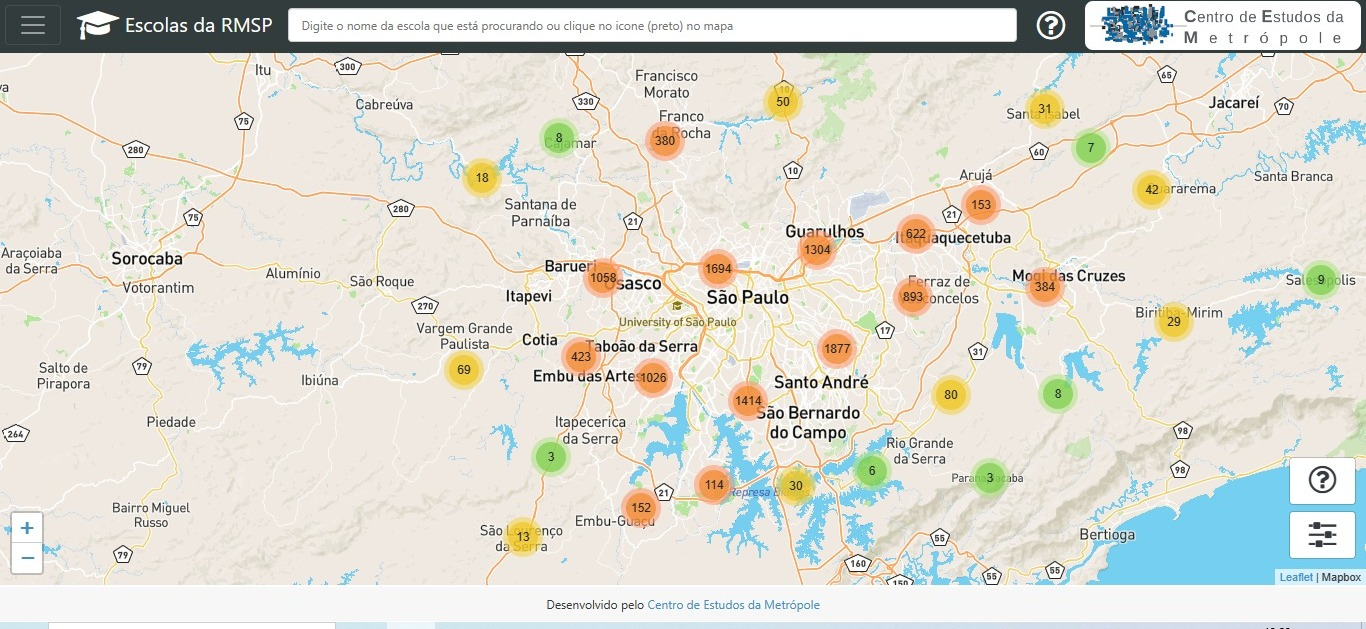
\includegraphics[width=0.8\textwidth]{Figuras/siteCEM.jpeg}
    \caption{Mapa de clusters do Centro de Estudos da Metrópole}
    \label{fig:siteCEM}
\end{figure} 

Apesar de o mapa de cluster ser uma representação útil, resolvemos criar um gráfico de pontos para melhor visualizar a distribuição dos dados de São Paulo e também para comparar de forma equivalente com a segunda base utilizada. A Figura \ref{fig:baseSP} mostra o gráfico citado. No gráfico também foi incluído o contorno da cidade de São Paulo para vizualizar a distribuição de endereços dentro e fora da cidade.

\begin{figure} 
    \centering
    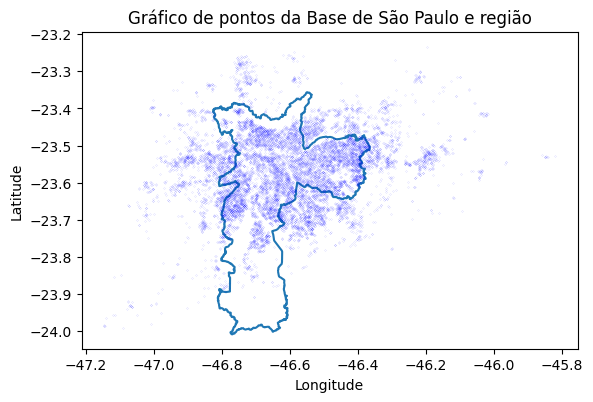
\includegraphics[width=0.8\textwidth]{Figuras/spCompleta.png}
    \caption{Gráfico de Endereços da Base de São Paulo e região metropolitana}
    \label{fig:baseSP}
\end{figure}

A segunda base de dados utilizada é fornecida pela \cite{Prodabel}, a empresa de informática e informação da prefeitura de Belo Horizonte. A descoberta dessa base de dados foi possibilitada pelo artigo de referência \cite{Clodoveu2011}. Essa base de dados é mantida e atualizada mensalmente por 27 empresas, tanto públicas quanto privadas, de Belo Horizonte. Essas empresas tem a responsabilidade de relatar quaisquer inconsistências encontradas na base e de fornecer novos dados à medida que os adquiriam. Ela é considerada uma fonte confiável de informações, pois está em constante atualização e é amplamente utilizada por diversos serviços da prefeitura. Um exemplo notável e é o uso da base para georreferenciamento na distribuição de alunos da rede pública. Esse serviço consiste em designar a escola pública para qual aluno irá com base na distância entre a moradia do aluno e a escola. Essa base então é utilizada para selecionar escolas para todos os alunos de forma a diminuir as distâncias entre a escola e os alunos para cada um dos alunos. Sendo assim, é uma base bastante relevante para a cidade de Belo Horizonte \cite{Clodoveu2011}.

Na data de acesso, essa base continha um total de 763.229 endereços. A prefeitura disponibiliza um \href{https://bhmap.pbh.gov.br}{site com um mapa} que permite a visualização desses endereços. A Figura \ref{fig:siteProdabel} mostra esse site, e na barra de pesquisa, os usuários podem pesquisar endereços específicos e marcá-los no mapa. É importante notar que, ao contrário da maioria das APIs de geocodificação, todos os endereços foram posicionados em cima dos edifícios representados. A discrepância entre essa abordagem e a prática comum de colocar o endereço na frente do edifício pode causar um pequeno erro de alguns metros na comparação da geocodificação.

\begin{figure}
    \centering
    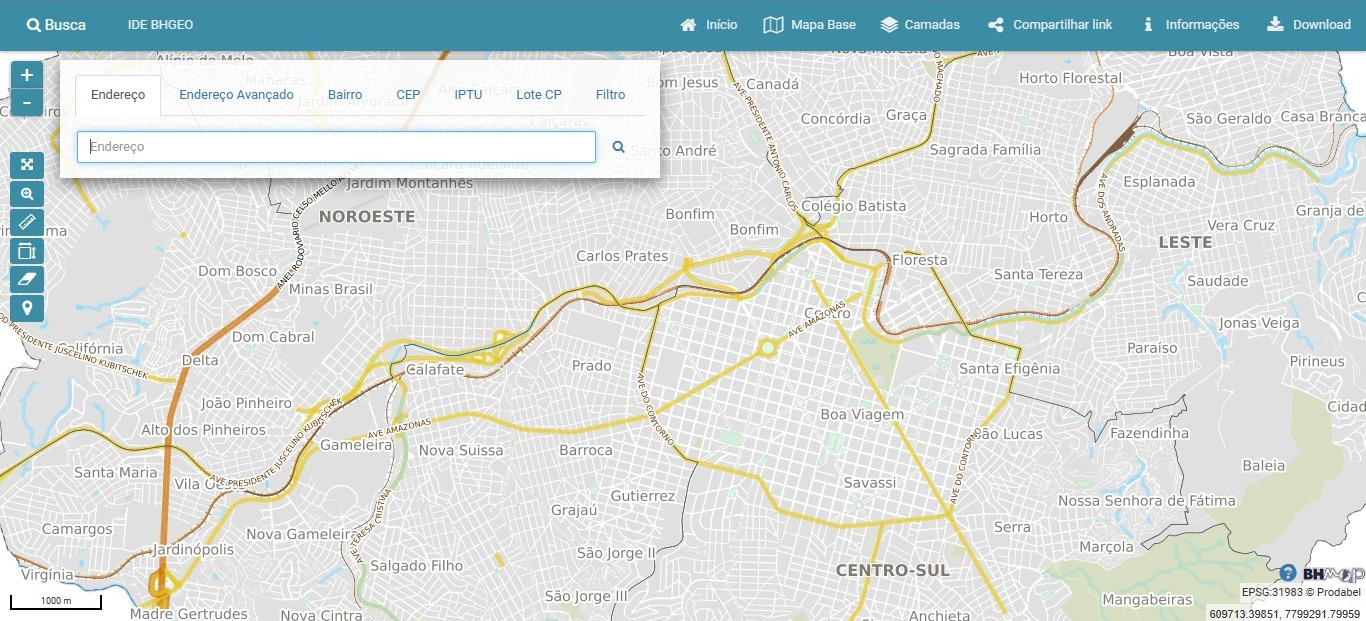
\includegraphics[width=0.8\textwidth]{Figuras/siteProdabel.jpeg}
    \caption{Site da Prodabel para pesquisa de endereços. }
    \label{fig:siteProdabel}
\end{figure}

Devido a limitações computacionais tanto dos autores deste trabalho quanto da aplicação responsável pela geocodificação, optamos por realizar uma amostragem da base de Belo Horizonte, com o intuito de reduzir a quantidade de dados processados. Nossa amostra consiste em 85.000 endereços da cidade. A fim de garantir uma distribuição uniforme dos endereços no espaço, empregamos o método do hipercubo latino para a amostragem. A Figura \ref{fig:baseBh} apresenta dois gráficos contendo os pontos da base original e os da amostra obtida. Os gráficos contém os pontos referentes a cada uma das bases e um contorno da cidade de Belo Horizonte. Com essa vizualização, é possível ver a concentração e cobertura dos pontos. É possível observar que a amostra cobre toda a área abrangida apesar de não ter tanta concentração de pontos quanto a base original. Além disso, verifica-se uma ligeira concentração nas regiões periféricas do desenho, permitindo uma melhor delimitação da cidade.

\begin{figure}[ht]
    \centering
    \begin{subfigure}[b]{0.45\textwidth}
      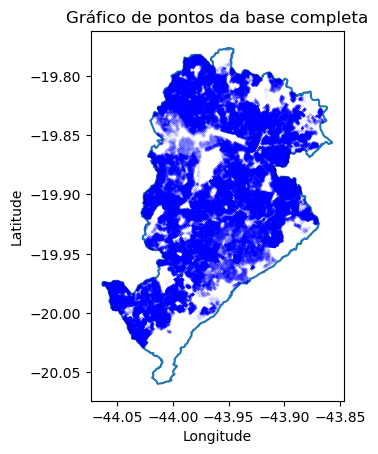
\includegraphics[width=\textwidth]{Figuras/bhCompleta.png}
      \caption{Completa}
      \label{fig:baseBhC}
    \end{subfigure}
    \hfill
    \begin{subfigure}[b]{0.45\textwidth}
      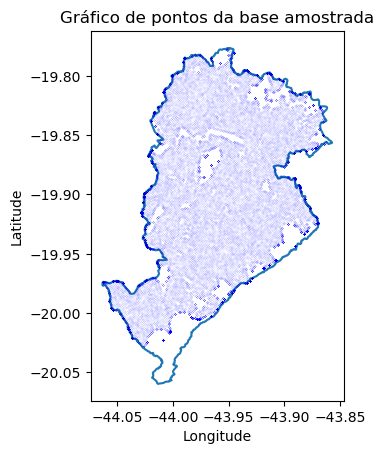
\includegraphics[width=\textwidth]{Figuras/bhAmostra.png}
      \caption{Amostra}
      \label{fig:baseBhA}
    \end{subfigure}
    \caption{Gráficos dos endereços da Base de Belo Horizonte e amostragem obtida}
    \label{fig:baseBh}
\end{figure}

\section{Processo de Geocodificação}
\label{processoGeo}

Após a coleta das bases, é necessário prepará-las para a geocodificação. A etapa de preparação de dados envolve a seleção dos campos relevantes da base de dados, como nome da rua, número, bairro, CEP e cidade. Em outras palavras, serão selecionados apenas os campos descritivos do endereço e os campos de localização geográfica do endereço. Após a seleção, os dados foram homogeneizados, substituindo abreviações comuns por suas formas completas correspondentes, e todas as letras foram transformadas em letras maiúsculas. A tabela \ref{tab:abreviacoes} do anexo \ref{tabela_abrev} contém as abreviações utilizadas no processo de padronização. Quaisquer abreviações não contidas na tabela não são tratadas. 

Para realizar a geocodificação, os endereços previamente preparados são inseridos no banco de dados da aplicação responsável por solicitar e coletar informações de geocodificação. Os endereços são então retirados desse banco para serem geocodificados. É importante destacar que o processo de geocodificação é executado pela equipe de Back-end do TerraLAB, e, portanto, é considerado um processo de "caixa preta".

Após a conclusão da geocodificação, os endereços geocodificados, juntamente com suas coordenadas geográficas, são armazenados no mesmo banco de dados, mas em tabelas distintas. A Figura \ref{fig:diagramaMono} esquematiza todo esse processo essencial para o nosso trabalho.

\begin{figure}
    \centering
    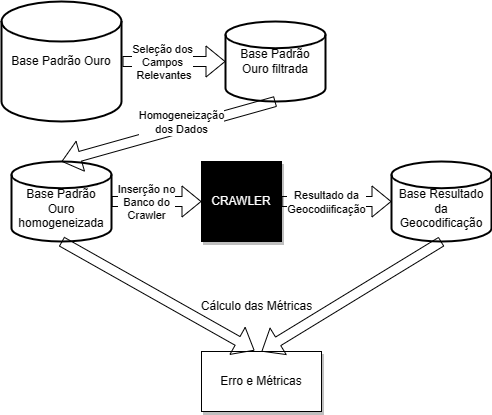
\includegraphics[width=0.8\textwidth]{Figuras/diagrama monografia.drawio.png}
    \caption{Esquematização do processo de preparação e geocodificação dos dados}
    \label{fig:diagramaMono}
\end{figure}

\section{Método de Avaliação}
\label{metricasErro}

\subsection{Erro e Taxa de Resposta}

A principal métrica utilizada para avaliar a qualidade da geocodificação é o erro do endereço. Com base nesse erro, calcularemos as medidas estatísticas média, mediana, desvio padrão média aparada em 5\%, para analisar a precisão das GeoAPIs. Esse erro é calculado como a distância entre o ponto de referência e o ponto geocodificado pela GeoAPI, conforme as equações abaixo:

\begin{equation}
e = D(p_{\text{Ouro}}, p_{\text{Geo}})
\end{equation}

Onde:
\begin{itemize}
\item $e$ é o erro da geocodificação,
\item $D$ é uma função que calcula a distância em quilômetros,
\item $p_{\text{Ouro}}$ é o ponto da base padrão ouro, e
item $p_{\text{Geo}}$ é o ponto resultante da geocodificação.
\end{itemize}

\begin{equation}
D( p_1(\text{lat}_1, \text{lon}_1), p_2(\text{lat}_2, \text{lon}_2) ) = \sqrt{{(\text{lat}_2 - \text{lat}_1)^2 + (\text{lon}_2 - \text{lon}_1)^2}}
\label{eq:distEuclidian}
\end{equation}

Onde:
\begin{itemize}
    \item $D$ é a distância euclidiana entre dois pontos,
    \item $p_1$ é o primeiro ponto,
    \item $p_2$ é o segundo ponto,
    \item $\text{lat}_1$ e $\text{lat}_2$ são as latitudes de $p_1$ e $p_2$, respectivamente,
    \item $\text{lon}_1$ e $\text{lon}_2$ são as longitudes de $p_1$ e $p_2$, respectivamente.
\end{itemize}

Além disso, outra métrica utilizada para avaliar a qualidede é a taxa de resposta da API. Para alguns endereços da base de dados, as GeoAPIs podem retornar um erro, não fornecendo uma geocodificação válida. A taxa de resposta é calculada como a quantidade de endereços geocodificados dividida pela quantidade de endereços originais na base de dados. Esse valor é convertido em uma porcentagem para facilitar a compreensão dos resultados, de acordo com a seguinte fórmula:

\begin{equation}
tx_{\text{resposta}} (\%) = \left(\frac{qtd_{\text{Geo}}}{qtd_{\text{Ouro}}}\right) \times 100\%
\end{equation}

Onde:
\begin{itemize}
    \item $tx_{\text{resposta}}$ é a taxa de resposta da API avaliada;
    \item $qtd_{\text{Ouro}}$ é a quantidade de endereços da base referência;
    \item $qtd_{\text{Geo}}$ é a quantidade de endereços resultantes da geocodificação.
\end{itemize}

Outra métrica obtida por meio do erro é a taxa de precisão. É definida como a porcentagem de endereços com um erro inferior a 150 metros em relação ao número total de endereços. Esse valor foi escolhido com base em \cite{Clodoveu2011}, que afirma que  150 metros é aproximadamente o tamanho de um quarteirão em Belo Horizonte. É representada pela seguinte fórmula:

\begin{equation}
tx_{\text{precisão}} (\%) = \left(\frac{qtd_{\text{certo}}}{qtd_{\text{Ouro}}}\right) \times 100\%
\end{equation}

 Onde:
 \begin{itemize}
     \item $tx_{\text{precisão}}$ é a taxa de precisão da API avaliada;
     \item $qtd_{\text{certo}}$ é a quantide de endereços em que o erro foi menor que 150 metros;
     \item $qtd_{\text{Ouro}}$ é a quantidade de endereços da base referência;
 \end{itemize}

\subsection{Discrepância}
 
Para encontrar uma medida que se compare ao erro utilizando apenas informações fornecidas pela geocodificação, é necessário avaliar a discrepância entre as geocodificações. Para isso, será utilizada a métrica de distância do ponto médio. Na distância até o ponto médio, computamos um ponto médio a partir de todas as geocodificações fornecidas para um endereço e então calculamos a distância euclidiana de uma geocodificação até esse ponto médio.

A distância até o ponto médio é calculada como a distância euclidiana de uma geocodificação até o ponto médio e é definida como:
 \begin{equation}
     \text{Distância até o Ponto Médio para cada ponto} = \sqrt{(\text{lat}_i - \text{mid\_lat})^2 + (\text{lon}_i - \text{mid\_lon})^2}
 \end{equation}
 
Onde:
 \begin{itemize}
     \item $\text{lat}_i$ e $\text{lon}_i$ são as latitudes e longitudes das geocodificações individuais,
     \item $\text{mid\_lat}$ e $\text{mid\_lon}$ são a latitude e longitude do ponto médio calculado.
 \end{itemize}

Para calcular o ponto médio entre os pontos do mesmo endereço de várias APIs, usamos a seguinte fórmula:

\begin{equation}
     \text{Ponto Médio} = \left(\frac{{\sum_{i=1}^{n} \bar{\text{lat}_i}}}{n}, \frac{{\sum_{i=1}^{n} \bar{\text{lon}_i}}}{n}\right)
\end{equation}

Onde:
 \begin{itemize}
     \item $\bar{\text{lat}_i}$ e $\bar{\text{lon}_i}$ representam a média de latitude e longitude para os mesmos endereços,
     \item $n$ representa o número de APIs.
 \end{itemize}

Para calcular a relação entre a discrepância e erro utilizaremos uma media de correlação e a medida escolhida foi a correlação de Pearson. A correlação de Pearson é uma medida de correlação descrita pela fórmula \cite{callegari2007}:

\[
 r = \frac{\sum_{i=1}^{n} (x_i - \bar{x})(y_i - \bar{y})}{\sqrt{\sum_{i=1}^{n} (x_i - \bar{x})^2 \sum_{i=1}^{n} (y_i - \bar{y})^2}}
\]

 onde:
 \begin{itemize}
     \item \(r\) é o coeficiente de correlação de Pearson;
     \item \(x_i\) e \(y_i\) são as variáveis avaliadas;
     \item \(\bar{x}\) e \(\bar{y}\) são as médias dos valores \(x\) e \(y\), respectivamente.

 \end{itemize}

 Essa medida, independente dos valores das variáveis sempre retorna um valor entre -1 e 1, sendo 1 uma correlação forte positiva e -1 uma correlação forte negativa. Quanto mais próximo de 0, menos correlação as variáveis tem. A tabela \ref{tab:correlacaoPearson} retirada do livro mostra para cada faixa de valor resultante da correlação de Pearson respectivos significados \cite{callegari2007}. É interessante portanto encontrar relações com  módulo do coeficiente superior a 0.6.

\begin{table}[ht]
 \centering
 \caption{Tabela de Correlação de Pearson}
 \label{tab:correlacaoPearson}
 \begin{tabular}{|c|c|}
 \hline
 $|r|$ & A correlação é dita \\
 \hline
 $0$ & Nula \\
 $0 - 0.3$ & Fraca \\
 $0.3 - 0.6$ & Regular \\
 $0.6 - 0.9$ & Forte \\
 $0.9 - 1$ & Muito Forte \\
 $1$ & Plena ou Perfeita \\
 \hline
 \end{tabular}
\end{table}

\section{Experimentos para avaliação da formatação da entrada}

Como mencionado anteriormente, algumas APIs disponilizam recomendações de formatações de entrada em suas documentações. A Tabela \ref{tab:tabelaEntradas} apresenta o formato recomendado para cada uma das APIs utilizadas, enquanto a Tabela \ref{tab:tabelaFormatos} especifica os formatos citados. 

\begin{table}[ht]
 \centering
 \caption{Formato Recomendado de Entrada para APIs de Geocodificação}
 \label{tab:tabelaEntradas}
 \begin{tabular}{|l|l|p{4cm}|}
 \hline
 API & Formato Recomendado & Documentação \\
 \hline
 Google Maps & \makecell{Recomenda utilizar o formato do \\ serviço postal do país buscado} & \cite{GoogleDoc}  \\
 \hline
 Open Route Service & \makecell{Sem recomendações específicas} & \cite{ORSdoc}  \\
 \hline
 Mapbox & \makecell{Recomenda utilizar o formato oficial dos EUA \\ ou o formato do serviço postal do país buscado} & \cite{MapboxDoc}  \\
 \hline
 TomTom & \makecell{Sem recomendações específicas} & \cite{TomtomDoc}  \\
 \hline
 \end{tabular}
\end{table}

\begin{table}[ht]
 \centering
 \caption{Descrição dos formatos}
 \label{tab:tabelaFormatos}
 \begin{tabular}{|c|c|}
 \hline
 Origem & Formato \\
 \hline
 Serviço postal do Brasil  & \makecell{\\Tipo de Logradouro, Nome do Logradouro, \\ Número do Lote, Complemento (se houver), \\ Nome do Bairro, Nome da Localidade, \\ Sigla da Unidade da Federação, CEP} \\
 \hline
 EUA & \makecell{Número do lote, Nome do Logradouro \\ Nome da Cidade, Nome do Estado, CEP} \\
 \hline
 \end{tabular}
\end{table}

Apesar disso, a equipe do TerraLAB tem seus próprio padrão de formatação utilizado. A Tabela \ref{tab:tabelaEntradasTerraLab} apresenta os formatos de entrada utilizados por cada uma das APIs no laboratório.

\begin{table}[ht]
    \centering
    \caption{Formato de Entrada das APIs Utilizadas pelo TerraLAB}
    \label{tab:tabelaEntradasTerraLab}
    \begin{tabular}{|c|c|}
    \hline
    API & Formato \\
    \hline
    Mapbox &  \makecell{Estado, Cidade, Número Lote, Tipo Logradouro, Nome Logradouro}\\
    \hline
    TomTom & \makecell{Tipo Logradouro, Nome Logradouro, Número do Lote, Cidade, Estado} \\
    \hline
    Google & \makecell{Tipo Logradouro, Nome Logradouro, Número do Lote, Cidade, Estado} \\
    \hline
    ORS  & \makecell{Tipo Logradouro, Nome Logradouro, Número do Lote, Cidade, Estado} \\
    \hline
    \end{tabular}
\end{table}

Para avaliar qual seria a melhor formatação dos dados de entrada, contruímos para cada API 5 experimentos onde são modificadas as ordens da palavra de entrada da API. A tabela \ref{tab:experimentosFormatos} mostra qual é o formato para cada um dos experimentos. Os experimentos foram numerados, durante o trabalho iremos nos referir a eles de acordo com esse número.

\begin{table}[ht]
\centering
\caption{Formato de cada experimento}
\label{tab:experimentosFormatos}
\begin{tabular}{|c|c|}
\hline
Experimento & Formato \\
\hline
1 &  \makecell{Tipo Logradouro, Nome Logradouro, Número Edifício, Cidade, Estado}\\
\hline
2 &  \makecell{Cidade, Tipo Logradouro, Nome Logradouro, Número Edifício,  Estado}\\
\hline
3 &  \makecell{Estado, Cidade, Tipo Logradouro, Nome Logradouro, Número Edifício}\\
\hline
4 &  \makecell{Estado, Tipo Logradouro, Nome Logradouro, Número Edifício, Cidade}\\
\hline
5 &  \makecell{Cidade, Estado, Tipo Logradouro, Nome Logradouro, Número Edifício}\\
\hline
\end{tabular}
\end{table}

Devido a quantidade de experimentos, resolvemos fazer uma amostragem das duas bases de dados. Selecionamos 5 mil endereços de cada base, utilizando o método de hipercubo latino. E utilizando o mesmo processo de padronização e geocodificação explicado na seção \ref{processoGeo}, obtivemos a geocodificação de cada uma das APIs para cada endereço. 

A base de Belo Horizonte continha as informações de bairro de cada endereço, diferente da base de São Paulo. Com isso, decidimos realizar uma análise adicional, que consistia em verificar se há algum ganho em adicionar o bairro na entrada. Portanto, para a base de Belo Horizonte forma adicionados 5 experimentos adicionais. A tabela \ref{tab:experimentosBairroFormatos} mostra os formatos citados.

\begin{table}[ht]
    \centering
    \caption{Formato dos experimentos adicionais}
    \label{tab:experimentosBairroFormatos}
    \begin{tabular}{|c|c|}
    \hline
    Experimento & Formato \\
    \hline
    1b &  \makecell{Tipo Logradouro, Nome Logradouro, Número Edifício, Bairro, Cidade, Estado}\\
    \hline
    2b &  \makecell{Cidade, Tipo Logradouro, Nome Logradouro, Número Edifício, Bairro, Estado}\\
    \hline
    3b &  \makecell{Estado, Cidade, Bairro, Tipo Logradouro, Nome Logradouro, Número Edifício}\\
    \hline
    4b &  \makecell{Estado, Tipo Logradouro, Nome Logradouro, Número Edifício, Bairro, Cidade}\\
    \hline
    5b &  \makecell{Cidade, Estado, Bairro, Tipo Logradouro, Nome Logradouro, Número Edifício}\\
    \hline
    \end{tabular}
\end{table}

Com as Geocoficações prontas, faremos o calcúlo das metricas de erro para cada uma das APIs, como explicado na seção \ref{metricasErro}. 